%!TEX program = xelatex
\documentclass[a4paper]{article}
\usepackage{fontspec}\defaultfontfeatures{Ligatures=TeX}
% \usepackage{setspace}\setstretch{1.3} % \begin{spacing}{1.3}
\usepackage[a4paper,vmargin={4cm,4cm},hmargin={4cm,4cm}]{geometry}
%-----------------------------------------------------------------------------%
\usepackage{settings}
%-----------------------------------------------------------------------------%
%%% Title %%%
\title{Shannon Entropy: Source Coding Problem%
\thanks{This introduction draws heavily from lecture note \textcite{duchi-2023}, Chapter 2.}%
}
\author{\href{https://jessekelighine.com}{jessekelighine.com}\\Jesse C.\ Chen\ 陳\,捷}
\date{\today}
%-----------------------------------------------------------------------------%

\begin{document}

\maketitle

\section{Motivation}

% In the age of computers,
% we naturally think of bits and bytes when discussing information,
% as ones and zeros are used to encode files.
% A file contains more information if more bits are required to encode its contents.
% Hence, a natural conception of \emph{information} is in terms of the length of its encoding.

Let $\mathcal{X}$ be a finite sample space,
and let $X$ be a random variable with $\pr$ as the induced probability measure on $\mathcal{X}$.
How much \emph{information} does $X$ carry?
We can approach this question as follows:
If we encode each possible outcome in $\mathcal{X}$ using a given set of symbols,
on average, what is the number of symbols required to represent a realization of $X$?

\begin{example}\label{eg:dice}
    Suppose we have a rigged six-sided die with the following probabilities and encoding in binary (two symbols):
    \begin{center}
        \begin{tabular}{crr}
            \toprule
            Face & Probability & Encoding \\
            \midrule
            $\dice{1}$ & $80\%$  & \texttt{1} \\
            $\dice{2}$ & $10\%$  & \texttt{01} \\
            $\dice{3}$ & $2.5\%$ & \texttt{0011} \\
            $\dice{4}$ & $2.5\%$ & \texttt{0010} \\
            $\dice{5}$ & $2.5\%$ & \texttt{0001} \\
            $\dice{6}$ & $2.5\%$ & \texttt{0000} \\
            \bottomrule
        \end{tabular}
    \end{center}
    Since it is highly probable that $\dice{1}$ will occur,
	it is efficient to assign it a short codeword.
	Under this scheme, 1.4 bits is expected to encode an outcome since
	\begin{align*}
		0.8 \times 1\text{ bit} + 0.1 \times 2\text{ bits} + (0.025 \times 4\text{ bits})\times 4 = 1.4 \text{ bits.}
	\end{align*}
    If the die is so rigged that only $\dice{1}$ ever occurs,
	then the die carries no information,
	as the outcome is entirely predictable.
	In this case, the required encoding length would be $0$ bits.
\end{example}

In the following sections,
we will formalize this idea of information through encoding
and derive Shannon entropy as a quantitative measure of information.

\section{Code Function}

\begin{definition}[$d$-ary Code Function]
	A \emph{$d$-ary code function} $\mathsf{C}$ maps
	$x\in\mathcal{X}$ to a finite string, denoted by $\mathsf{C}(x)$, consisting of $d$ distinct symbols.
	% say $\{0,...,d-1\}$.
	The output of $\mathsf{C}$ is referred to as the \emph{codeword}.
	Codewords can have different lengths
	and let $\ell_{\mathsf{C}}(x)$ denote the length of the codeword used to encode $x\in\mathcal{X}$.
\end{definition}

% \begin{example}\label{eg:ascii}
% 	Perhaps the simplest code function is a binary one, i.e., $d=2$.
% 	If $\mathcal{X}$ is the set of alphabets,
% 	a code function can be the ASCII encoding.
% 	So letter \texttt{A} is mapped to \Verb"01000001", \texttt{B} to \Verb"01000010", etc.
% 	And with ASCII encoding, $\ell_{\mathsf{C}}(x)=8$ for any $x\in\{\mathtt{A},...,\mathtt{Z}\}$.
% \end{example}

\begin{remark}
	For any $d$-ary code function $\mathsf{C}$ to be considered reasonable,
	it must allow the encoded message to be decoded unambiguously.
	This requires certain properties to hold, as defined below.
	% we must be able to ``decode'' the message encoded by $\mathsf{C}$.
	% The following are two obvious properties a reasonable $\mathsf{C}$ must possess.
\end{remark}

\begin{definition}[Non-singular]
	A $d$-ary code function $\mathsf{C}$ is \emph{non-singular}
	if for all $x,x'\in\mathcal{X}$, we have $\mathsf{C}(x) = \mathsf{C}(x')$ \text{iff} $x=x'$.
\end{definition}

\begin{definition}[Uniquely Decodable]
	A $d$-ary code function $\mathsf{C}$ is \emph{uniquely decodable}
	if for all sequences $x_1,...,x_n\in\mathcal{X}$ and $x_1',...,x_n'\in\mathcal{X}$,
	we have
	\begin{align*}
		\mathsf{C}(x_1)\cdots\mathsf{C}(x_n) = \mathsf{C}(x_1')\cdots\mathsf{C}(x_n')
		\quad\text{iff}\quad
		x_1=x_1',...,x_n=x_n'.
	\end{align*}
	That is, there is no ambiguity in any encoded sequences.
\end{definition}

\begin{remark}
	If a code function is uniquely decodable, then it must be non-singular,
	but not the other way round.
	A particularly useful type of uniquely decodable code is the \emph{prefix code}.
\end{remark}

% \begin{remark}
% 	The ASCII code is uniquely decodable
% 	simply because every alphabet is mapped to $8$ bits and each character has a unique mapping.
% 	However, it is not necessary that a uniquely decodable $\mathsf{C}$ maps every element $\mathcal{X}$ to strings of the same length.
% 	A particularly useful uniquely decodable encoding scheme is called \emph{prefix code}.
% \end{remark}

\section{Prefix Code}

\begin{figure}[t]
	% \centering
	% \begin{subfigure}{0.45\textwidth}
	% 	\centering
	% 	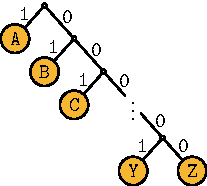
\includegraphics[scale=1]{figures/prefix-tree-ascii.pdf}
	% 	\caption{A to Z}
	% 	\label{fig:prefix-tree-ascii}
	% \end{subfigure}
	% \begin{subfigure}{0.45\textwidth}
		\centering
		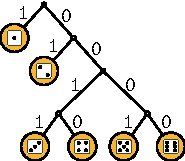
\includegraphics[scale=1]{figures/prefix-tree-dice.pdf}
		\caption{Prefix Tree: Dice.}
		\label{fig:prefix-tree-dice}
	% \end{subfigure}
	% \caption{Prefix Tree.}
	% \label{fig:prefix-tree}
\end{figure}

\begin{definition}[Prefix Code]
	A $d$-ary code function $\mathsf{C}$ is said to be a \emph{prefix code}
	if $\nexists c,c'\in\{\mathsf{C}(x)\}_{x\in\mathcal{X}}$ such that $c'$ starts with $c$.
	That is, no whole codeword is a prefix of any other codeword.
\end{definition}

\begin{remark}
	Since no codeword is the start of any other codeword,
	a prefix code can be represented by a graph called \emph{prefix tree}.
	And there is a one-to-one correspondence between prefix trees and prefix codes.
	The encoding given in \autoref{eg:dice} is a prefix code
	and the corresponding prefix tree is shown in \autoref{fig:prefix-tree-dice}.
\end{remark}

% \begin{example}\label{eg:prefix-code}
% 	Suppose a coding function $\mathsf{C}$ maps alphabets in the following manner:
% 	$\mathsf{C}(\mathtt{A}) = \mathtt{1}$,
% 	$\mathsf{C}(\mathtt{B}) = \mathtt{01}$,
% 	$\mathsf{C}(\mathtt{C}) = \mathtt{001}$,
% 	$\mathsf{C}(\mathtt{D}) = \mathtt{0001}$, etc.
% 	This is clearly a prefix code.
% 	This code is represented in \autoref{fig:prefix-tree-ascii} as a prefix tree.
% \end{example}

\begin{lemma}
	Any prefix code is uniquely decodable.
\end{lemma}
\begin{proof}
	This should be pretty obvious with the prefix tree representation.
\end{proof}

% \begin{remark}
% 	The ASCII code is a prefix code, so it is uniquely decodable.
% \end{remark}

\begin{remark}
	Prefix codes are among the simplest uniquely decodable codes to work with.
	While there are other uniquely decodable encoding schemes,
	prefix codes are special because of the \nameref{thm:kraft-mcmillan-inequality}.
\end{remark}

\begin{theorem}[Kraft-McMillan Inequality]\label{thm:kraft-mcmillan-inequality}
	Let $\mathcal{X}$ be a finite set,
	and let $\ell:\mathcal{X}\to\naturals$ be a function.
	If $\ell(x)$ is the length of the encoding of the element $x$ in a uniquely decodable $d$-ary,
	then
	\begin{align*}
		\sum_{x\in\mathcal{X}} d^{-\ell(x)} \leq 1.
	\end{align*}
	Conversely, given any function $\ell:\mathcal{X}\to\naturals$
	that satisfies the inequality above,
	there exists a prefix code $\mathsf{C}$ such that $\ell_{\mathsf{C}}(x)=\ell(x)$ $\forall x\in\mathcal{X}$.
\end{theorem}
\begin{proof}
	First suppose that $|\mathcal{X}|<\infty$.
	Let $\ell_{\text{max}}\coloneqq\max_{x\in\mathcal{X}}\ell(x)$ denote the longest codeword.
	Let $x_{1:n}\coloneqq(x_1,...,x_n)\in\mathcal{X}^n$.
	Define the notation
	\begin{align*}
		E_n(m) \coloneqq \{x_{1:n}:\ell(x_{1:n})=m\}
	\end{align*}
	where $\ell(x_{1:n})=\sum_{i=1}^n\ell(x_i)$.
	That is, $E_n(m)$ denotes the set of strings of $n$ elements in $\mathcal{X}$ that is encoded with $m$ symbols.
	Clearly, we have $\ell(x_{1:n})\leq n\ell_{\text{max}}$,
	and by unique decodability, we must have $|E_n(m)|\leq d^m$.
	Consider the following rewriting of the sum for any fixed $n$:
	\begin{align*}
		\sum_{x_{1:n}\in\mathcal{X}^n} d^{-\ell(x_{1:n})}
		= \sum_{m=1}^{n\ell_{\text{max}}} |E_n(m)| d^{-m}
		\leq \sum_{m=1}^{n\ell_{\text{max}}} d^{m} d^{-m}
		= n\ell_{\text{max}}.
	\end{align*}
	We can rewrite the sum in another way:
	\begin{align*}
		\sum_{x_{1:n}\in\mathcal{X}^n} d^{-\ell(x_{1:n})}
		= \sum_{x_{1:n}\in\mathcal{X}^n} d^{-\ell(x_1)} \cdots d^{-\ell(x_n)}
		= \left( \sum_{x\in\mathcal{X}} d^{-\ell(x)} \right)^{n}.
	\end{align*}
	Hence, for all $n$ we have
	\begin{align*}
		\sum_{x\in\mathcal{X}} d^{-\ell(x)}
		% = \left( \left( \sum_{x\in\mathcal{X}} d^{-\ell(x)} \right)^n \right)^{1/n}
		= \left( \sum_{x_{1:n}\in\mathcal{X}^n} d^{-\ell(x_{1:n})} \right)^{1/n}
		\leq (n\ell_{\text{max}})^{1/n}.
	\end{align*}
	Taking $\inf_{n\in\naturals}$ on both sides and we obtain the inequality.
	% For countable $\mathcal{X}$, let $\mathcal{X}_k\coloneqq\{x\in\mathcal{X}:\ell(x)\leq k\}$ and define
	% $D_k \coloneqq \sum_{x\in \mathcal{X}_k} d^{-\ell(x)}$.
	% Since $\mathcal{X}$ is unique decodable, each $\mathcal{X}_k$ is unique decodable.
	% Therefore, we have
	% \begin{align*}
	% 	\sum_{x\in\mathcal{X}} d^{-\ell(x)}
	% 	= \lim_{k\to\infty} \sum_{x\in \mathcal{X}_k} d^{-\ell(x)}
	% 	= \lim_{k\to\infty} D_k
	% 	\leq 1
	% \end{align*}
	% since $D_k\leq 1$ $\forall k$ by unique decodability of each $\mathcal{X}_k$.

	Now consider the converse.
	WLOG, let elements of $\mathcal{X}$ be a consecutive subset of $\naturals$ such that $\ell(x)\leq\ell(y)$ $\forall x\leq y$ starting from $1$.
	We place all the elements in a $d$-ary prefix tree as follows:
	First, place $1\in\mathcal{X}$ at a node of depth $\ell(1)$ and prune all the descendants from that node.
	This means that for an arbitrary $n\in\mathcal{X}$,
	there are $d^{\ell(n)-\ell(1)}$ nodes of depth $\ell(n)$ removed from the pruning.
	Then, we place $2\in\mathcal{X}$ at a node of depth $\ell(2)$,
	removing $d^{\ell(n)-\ell(2)}$ nodes of depth $\ell(n)$ from the prefix tree.
	This process continues until $n\in\mathcal{X}$ is placed in the tree.
	Note that this process never removes more nodes than there are available to us at any point $n$
	since the \nameref{thm:kraft-mcmillan-inequality} holds:
	\begin{align*}
		\sum_{i=1}^{n} d^{\ell(n)-\ell(i)}
		= d^{\ell(n)} \sum_{i=1}^{n} d^{-\ell(i)}
		\leq d^{\ell(n)}.
	\end{align*}
	Therefore, a prefix tree, hence a prefix code, can always be constructed by this method.
\end{proof}

\begin{remark}
	The \nameref{thm:kraft-mcmillan-inequality} characterizes unique decodability.
	Furthermore, it shows that we can always re-encode a uniquely decodable code function using a prefix code.
\end{remark}

\section{Entropy as Information}

\begin{definition}[Shannon Entropy]
	Let $X$ be a random variable with sample space $\mathcal{X}$.
	Define \emph{Shannon entropy} as
	\begin{equation*}
		\Eta_d(X) \coloneqq -\sum_{x\in\mathcal{X}} \pr(x) \log_d\pr(x)
	\end{equation*}
	where $\pr$ is the probability measure induced by $X$ on $\mathcal{X}$.
\end{definition}

\begin{remark}
	Note the negative sign in $\Eta_d(X)$.
	Since $\log\pr(x)$ is always non-positive, the negative sign keeps the entire thing non-negative.
	And by convention, for any $x\in\mathcal{X}$ such that $\pr(x)=0$, we define $\pr(x)\log_d\pr(x)=0$.
\end{remark}

\begin{remark}
	It turns out that the minimal average length of a codeword necessary to encode $X$ is given by $\Eta_d(X)$.
	This result is called \nameref{thm:shannon-source-coding}.
\end{remark}

\begin{theorem}[Shannon's Source Coding Theorem]\label{thm:shannon-source-coding}
	Let $X$ be a random variable with sample space $\mathcal{X}$.
	% and let $\pr$ denote the probability measure induced by $X$ on $\mathcal{X}$.
	Let $\mathcal{C}$ denote the set of all possible uniquely decodable $d$-ary code functions for $\mathcal{X}$.
	Then
	\begin{align*}
		\Eta_d(X)
		\leq \inf_{\mathsf{C}\in\mathcal{C}} \E \ell_{\mathsf{C}}(X)
		\leq \Eta_d(X) + 1
	\end{align*}
	where $\pr$ is the probability measure induced by $X$ on $\mathcal{X}$
	and $\E$ denotes the expectation operator.
\end{theorem}
\begin{proof}
	By \nameref{thm:kraft-mcmillan-inequality},
	solving $\inf_{\mathsf{C}\in\mathcal{C}}\E\ell_{\mathsf{C}}(X)$ is equivalent to solving
	\begin{align*}
		\inf_{\ell} \sum_{x\in\mathcal{X}} \pr(x) \ell(x)
		\quad\text{subject to}\quad
		\sum_{x\in\mathcal{X}} d^{-\ell(x)} \leq 1.
	\end{align*}
	This can be done by setting up and solving the Lagrangian:
	\begin{align*}
		\mathcal{L} = \sum_{x\in\mathcal{X}} \pr(x)\ell(x) + \lambda \left(1-\sum_{x\in\mathcal{X}}d^{-\ell(x)}\right)
		&\implies \pr(x) - \lambda d^{-\ell(x)}\log(d) \leteq 0\ \forall x \\
		&\implies \ell(x) = -\log_d \pr(x).
	\end{align*}
	Thus, the lower bound is obtained.
	For the upper bound, let $\ell(x)=\lceil-\log_d\pr(x)\rceil$.
	Note that this $\ell$ satisfies \nameref{thm:kraft-mcmillan-inequality},
	hence a prefix code can be constructed.
	Therefore, we have
	\begin{align*}
		\E\ell(X)
		= \sum_{x\in\mathcal{X}} \pr(x) \lceil-\log_d\pr(x)\rceil
		\leq \sum_{x\in\mathcal{X}} \pr(x) (-\log_{d}\pr(x)) + 1
		= \Eta_d(X) + 1,
	\end{align*}
	obtaining the upper bound.
\end{proof}

\begin{remark}
	For the rigged die in \autoref{eg:dice}
	the entropy is about $1.12$ bits.
	Our encoding scheme achieves an expected length of $1.4$ bits,
	which is close to the theoretical limit.
	There are also an asymptotic version of this theorem:
	If we observe a stationary sequence $X_1,X_2,...$,
	then we can re-encode the $X_i$'s in blocks.
	This way the expected length of encoding can be arbitrarily close to its entropy.
	One can refer to \textcite{duchi-2023}, Chapter 2 for the proof.
\end{remark}

\vfill
\printglossaries
\section*{References}
\printbibliography[heading=none]

\end{document}
